
%%%%%%%%%%%%%%%%%%%%%%%%%%%%%%%%%%%%%%%%%%%%%%%%%%%%%%%%%
% The original template for this document was taken from:
% http://www.michaelshell.org/tex/ieeetran/
%
% Adapted for courses at the University of Regina by:
% Mikhail Shchukin 
%
% Edited by Trevor Tomesh
% October 20th 2019
%%%%%%%%%%%%%%%%%%%%%%%%%%%%%%%%%%%%%%%%%%%%%%%%%%%%%%%%%

%!!!!!!!!!!!!!!!!!!!!!!!!!!!!!!!!!!!!!!!!!!!!!!!!!!!!!!!!
%!!!!!!!!!!!!! DON'T TOUCH THIS !!!!!!!!!!!!!!!!!!!!!!!!!
\documentclass[journal,onecolumn]{IEEEtran}
\usepackage{graphicx}
\usepackage{placeins}
\usepackage{mathtools}
\usepackage{listings}
\usepackage{threeparttable}
\usepackage{subfigure}
\graphicspath{ {./img/} }
\hyphenation{op-tical net-works semi-conduc-tor}
\begin{document}
%!!!!!!!!!!!!!!!!!!!!!!!!!!!!!!!!!!!!!!!!!!!!!!!!!!!!!!!!!
%!!!!!!!!!!!!!!!!!!!!!!!!!!!!!!!!!!!!!!!!!!!!!!!!!!!!!!!!!


% Enter the course, assignment number, your name, and student ID below: 
\newcommand{\course}{CS 490DB} % course
\newcommand{\anum}{6} % assignment number
\newcommand{\name}{Trevor M. Tomesh} % your name
\newcommand{\sid}{20012345} % student ID


%!!!!!! DON'T TOUCH THIS !!!!!!!!!!!!!!!!!!!!!!!!!!!!!!!!!!
\title{\course{} \\ Assignment \# \anum{}}
\author{\name{},~\IEEEmembership{\course{},~University~of~Regina},~Student ID\# \sid{}}
\maketitle
%!!!!!!!!!!!!!!!!!!!!!!!!!!!!!!!!!!!!!!!!!!!!!!!!!!!!!!!!!!


\section{Description}
This document is a write-up for assignment 6 in CS 490DB -- Applications in Natural Sciences. In this assignment, we have been asked to take 
raw data from the CDC's list of ``parasites of public health concern''~\cite{cdc:2019} and perform the following operations in a python program:

\begin{itemize}
\item read the raw data from a plain-text file into python
\item parse out the individual parasites from this raw data using a 
list comprehension
\item assign each parasite a number and a random ``type'' like a Pokemon
\item write the parasites out to a CSV in the following format: \emph{number, name, type}
\end{itemize}

While it was not required, I have decided to include exception handling on writing the CSV 
file because this tends to be the portion of the code that is most likely to fail given 
permissions issues. 

\section{User Interaction}
This is a command-line application with minimal user interaction. To use the program, a user only needs to write invoke the python3 interpreter as shown in Fig.~\ref{fig:success}.

\begin{figure}[h]
	\centering
  	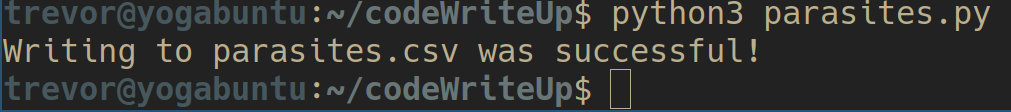
\includegraphics[width=0.5\textwidth]{img/success.png}
  	\caption{Basic User Interaction}	
  	\label{fig:success}
\end{figure}

If the program has run successfully, the user will receive the message \emph{``Writing to parasites.csv was successful!''}. However, if the program has not run successfully, the user
will receive the message \emph{``The following error occurred: ''} followed by the specific 
exception as shown in Fig.~\ref{fig:fail}. 

\begin{figure}[h]
	\centering
  	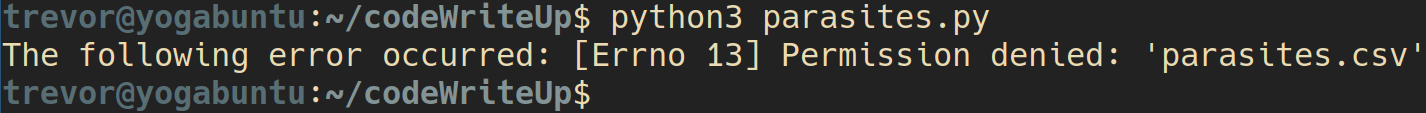
\includegraphics[width=0.5\textwidth]{img/fail.png}
  	\caption{Writing to CSV has failed}	
  	\label{fig:fail}
\end{figure}

\section{Known Issues and Limitations}
For some reason the program seems to put quotation marks around some of the parasite 
names and not around others. There should be no quotation marks around names other than ``crabs'' as it is the common nick-name for a parasite. Otherwise, the program meets all 
of the criteria listed so long as the text file is present in the same directory as the 
program and is not edited from its given state. 

\newpage

\appendices

\section{Answers to Assignment Questions}
\begin{enumerate}
	\item \emph{Q: Explain how a list comprehension works.} \\
	A: A list comprehension is analogous to a ``set builder'' in mathematics 
	whereby a list of output elements is constructed from a collection of input 
	elements (called the iterator) given some condition~\cite{yordanov:2019}. 
	For example: 

	\begin{lstlisting}[language=Python]
	numbers = [1, 2, 3, 4, 5]
	squares = [number**2 for number in numbers if number > 2]
	print(squares)
	\end{lstlisting}

	output:
 
	\begin{lstlisting}
	[9, 16, 25]
	\end{lstlisting}

	As illustrated above, the comprehension will take a number from the list ``numbers'' if that
	number is greater than 2 and add the square of that number to the list ``squares''. \\

    \item \emph{Q: What is the meaning of life, the universe and everything?} \\
    A: While the generally accepted answer is ``42'' as per author Douglas Adams~\cite{adams:1980}, Dr. Jordan Peterson argues that the meaning of life is to be found in the adoption of responsibility~\cite{lott:2019}. \\

    \item \emph{Q: What is your favorite sorting algorithm?} \\
    A: Merge Sort 

\end{enumerate}	

\newpage

\section{parasites.py}
\label{app1}
\lstset{basicstyle=\small\selectfont\ttfamily}
\lstinputlisting[language= python, 
breaklines=true,         
showtabs=false,
showstringspaces=false,
numberstyle=\tiny\color{mygray}
caption={The raw code for this assignment},
captionpos=b,label=lst2]{parasites.py}

\newpage

\section{parasites.txt}
\label{app1}
\lstset{basicstyle=\small}
\lstinputlisting[language= , breaklines=true,
caption={The raw input for the assignment},
captionpos=b,showstringspaces=false,label=lst3]{parasites.txt}

\newpage

\section{parasites.csv}
\label{app1}
\lstset{basicstyle=\ttfamily \small}
\lstinputlisting[language= , breaklines=true,
caption={The output for this assignment},
captionpos=b,showstringspaces=false,label=lst4]{parasites.csv}

\newpage

\begin{thebibliography}{1}


\bibitem{adams:1980}
Adams, Douglas, 1952-2001. ( 1980). \emph{The hitchhiker's guide to the galaxy.} New York :Harmony Books

\bibitem{cdc:2019}
CDC - DPDx - \emph{Parasites A-Z Index.} (2019). Retrieved 20 October 2019, from https://www.cdc.gov/dpdx/az.html

\bibitem{graham:2019}
Graham, D. (2019). \emph{Dunc's Regex} (Version 2). Regina.

\bibitem{lott:2019}
Lott, T. (2019). Jordan Peterson: ‘The pursuit of happiness is a pointless goal’. Retrieved 20 October 2019, from https://www.theguardian.com/global/2018/jan/21/jordan-peterson-self-help-author-12-steps-interview

\bibitem{yordanov:2019}
Yordanov, V. (2019). \emph{Python Basics: List Comprehensions.} Retrieved 20 October 2019, from https://towardsdatascience.com/python-basics-list-comprehensions-631278f22c40

\end{thebibliography}

% this is the end of all
\end{document}
